\documentclass[letterpaper, 10 pt, conference]{ieeeconf}
%\documentclass[a4paper, 10pt, conference]{ieeeconf}      % Use this line for a4 paper

\IEEEoverridecommandlockouts                              % This command is only needed if 
                                                          % you want to use the \thanks command

\overrideIEEEmargins  
%\usepackage[tmargin=2cm,lmargin=2cm,rmargin=2cm,bmargin=2.5cm]{geometry}
\usepackage[utf8]{inputenc}
\usepackage{cite}
\usepackage{graphicx} 
\usepackage{amsmath}
\usepackage{siunitx}
\usepackage{multirow}
%\usepackage{appendix}
\usepackage{comment} 
\usepackage{authblk}
\usepackage{algorithmicx}
%\usepackage{algorithm}% http://ctan.org/pkg/algorithm
\usepackage[ruled]{algorithm2e}% http://ctan.org/pkg/algorithmicx
%\usepackage{caption}
%\usepackage{subcaption}
\usepackage[table]{xcolor}
\usepackage{lettrine}
\usepackage{url}
\usepackage{authblk}
\usepackage{amsfonts}
\usepackage{bm}
\let\proof\relax
\let\endproof\relax
\usepackage{amsthm}
\usepackage[english]{babel}
\usepackage{amssymb}

\newtheorem{theorem}{Theorem}
\newtheorem{lemma}[theorem]{Lemma}

\allowdisplaybreaks[4]
\newcommand\mcedit[1]{\textcolor{black}{#1}}
\newcommand\mdsedit[1]{\textcolor{black}{#1}}
\newcommand\mccheck[1]{\textcolor{black}{#1}}
\newcommand\mbedit[1]{\textcolor{black}{#1}}
\title{\LARGE \bf
DC-TMPC: A tube-based MPC algorithm for nonlinear systems that can be expressed as a difference of convex functions.
}


\author[$\star$]{Martin Doff-Sotta}% <-this % stops a space
\author[$\star$]{Mark Cannon}

\affil[$\star$]{Control Group, University of Oxford}


\begin{document}


\maketitle
%\thispagestyle{empty}
\pagestyle{plain}

\begin{abstract}
We propose DC-TMPC, a novel robust tube-based model predictive control paradigm for nonlinear systems whose dynamics can be expressed as a difference of convex functions. The approach relies on successively perturbing the system predicted trajectories and bounding the linearisation error by exploiting convexity of the system dynamics. The linearisation error is then treated as a disturbance of the perturbed system to construct robust tubes containing the predicted trajectories, enabling the robust nonlinear MPC optimisation to be performed in  real time as a sequence of convex optimisation programs. Convergence, recursive feasibility and stability of the proposed approach are demonstrated. A case study involving a coupled tank problem is presented to illustrate an application of the algorithm. \\

\noindent\textbf{Keywords:}
Tube-based MPC, nonlinear MPC, robust MPC, Convex optimisation.
\end{abstract}

\section{Introduction}
\lettrine{R}{obust} model predictive control (MPC) is concerned with preserving performances and closed-loop stability properties in the presence of uncertainty \cite{kouvaritakis}, while offering the optimality, real-time tractability and constraint satisfaction of classical MPC. These methods are based on the idea that the knowledge of a set bounding the uncertainty in the dynamics allows one to define a sequence of sets to which the system future inputs and states converge \cite{kouvaritakis}.

Tube-based MPC is a specialised robust MPC technique that conveniently relies on a parameterisation of the uncertainty sets in terms of a tube in which the system trajectories are guaranteed to remain. A tube is made of a sequence of sets which contain the system states and inputs at a future instant for all realisations of the uncertainty \cite{kouvaritakis}. %Robust stabilisation of the system trajectory $x_k$ into a tube is made possible via a two-degree-of-freedom controller $u_k = c_k + \kappa(x_k, x^0_k)$. On the one hand, a feedforward control sequence $c_k$ is computed to stabilise the system around a nominal trajectory $x^0_k$. It is derived online by minimisation of an optimisation cost for the nominal system subject to tightened constraint sets that account for the presence of bounded disturbances. On the other hand, a state feedback controller $\kappa(x_k, x^0_k)$ is designed to steer the system inside the uncertainty sets. 
%
Tube-based MPC has been successfully applied to robustly stabilise linear systems \cite{gossner1997stable, schuurmans2000robust, lee1999constrained, chisci2001systems, goulart, langson2004robust, rakovic2012homothetic, mayne2005robust}. %See \cite{kouvaritakis} or \cite{rawling} for a modern treatment.

Application of tube-based MPC to nonlinear systems poses a series of challenges: online solution of a non-convex optimisation problem, safe approximation of uncertainty sets for states described by nonlinear dynamic equations, complexity associated with searching for a general nonlinear control policy, to name but a few. An early implementation of robust MPC to nonlinear uncertain systems was proposed in \cite{mayne2007tube} with a tube MPC  framework, and relying on the concept of constraint tightening as introduced in \cite{michalska1993robust}. %The control law is computed using two successive MPC controllers: on the one hand, the central line of the tube is obtained by minimising a nominal cost subject to nonlinear dynamics and tightened constraint sets, while on the other hand, an ancillary MPC law is used to reject the disturbances acting on the system and maintain the trajectory within sets of known size centred along the tube line. Computation of the tightened constraint sets is more difficult in the nonlinear case because the system describing the evolution of the error is no longer autonomous and the error is thus less easily bounded \cite{rawling}.

Sometimes, the special structure of the dynamics can be exploited to good advantage to define a nonlinear tube MPC framework. In \cite{rakovic2006simple}, a method is proposed for nonlinear systems with input-matched nonlinearities and nonlinear processes that take the form of piecewise affine maps. Feedback linearisation is used to cancel nonlinearities and a two-degree-of-freedom linear control law stabilises the system trajectory in a tube formed by robustly invariant sets. A method is proposed in \cite{yu2013tube} to construct robust invariant sets for a class of Lipschitz nonlinear systems, relying on the computation of a quadratic Lyapunov function and associated state feedback controller. In practice, such approach is limited since finding a global Lipschitz constant may result in a conservative controller with poor performance. Nonlinear system dynamics with a differential flatness property can also be advantageously reformulated to define a tube-based receding-horizon controller as in \cite{petkar2016robust}.

A common strategy in nonlinear tube-based MPC is to treat the nonlinearity in the dynamics as a bounded disturbance \cite{lee2002constrained, althoff2008reachability, cannon2009successive, mark}. In \cite{mark}, successive linear approximations around predicted trajectories are used to obtain a MPC law for a class of nonlinear systems. The proposed algorithm uses bounds on the  successive linearisation error of the system to construct a tube and associated controller. The controller achieves rejection of the linearisation error and stabilisation of the nonlinear system within a tube formed with  ellipsoidal sets with time-varying sizes. Asymptotic stability under the control law is demonstrated.

Although computationally tractable, these approaches rely on overly conservative bounds on the linearisation error, which are computed using fixed bounds on the predicted future states. In this work, we show that under some convexity assumptions, tighter bounds can be obtained. We consider systems that can be expressed as a difference of convex functions. A convex nonlinear function developed as a Taylor series truncated to the first order term has a convex  linearisation error.  For convex  linearisation errors defined on compact sets, the maximum occurs at the boundary of the domain, and the minimum is zero, which allows to construct non-conservative bounds for the error. If the error is treated as a disturbance of the perturbed dynamics, the tube-based MPC formalism can be applied efficiently to robustly stabilise the nonlinear system in real time. 

The paper is organised as follows. After a quick theoretical reminder on notations and successive linearisation tube-based MPC in Sections  \ref{sec:notations} and \ref{sec:TMPC}, Section \ref{sec:theory} presents the theory for the new DC-TMPC controller. Demonstrations of the convergence, stability and feasibility properties of the algorithm are presented in Section  \ref{sec:convergence}. Finally, the controller is applied to the regulation of a coupled tank in Section \ref{sec:case} as a case study. 

\section{Notations}
\label{sec:notations}
Let $x[n] = x(n\delta) \in  \mathbb{R}^{n_{x}}$, $\forall n \in \mathbb{N}$ be a discrete-time variable sampled at $t=n\delta$, using a step of $\delta$. The notation $\{ x_{0} , x_{1} , \ldots x_{N-1}\}$ is used for the sequence of current and future values of the variable $x$ predicted at the $n$th discrete-time step, so that $x_k$ denotes the predicted value $x_{n+k|n}$ or $x\bigl((n+k)\delta\bigr)$.\\

Let $\mathcal{S}_1$ and $\mathcal{S}_2$ be two subsets of $\mathbb{R}^{n_{x}}$. The Minkowski set addition operation is defined by $\mathcal{S}_1 \oplus \mathcal{S}_2 := \{s_1 + s_2 : s_1 \in \mathcal{S}_1, s_2 \in \mathcal{S}_2\}$. The set subtraction is defined by $\mathcal{S}_1 \ominus \mathcal{S}_2 :=  \{x \in \mathbb{R}^{n_{x}}: \{x\} \oplus  \mathcal{S}_1 \subseteq \mathcal{S}_2\}$. Let $K \in \mathbb{R}^{m \times n}$, the set multiplication operation is defined by $ K \mathcal{S}_1 := \{K s_1 : s_1 \in \mathcal{S}_1 \}$. The notation $\{x\}$ denotes the set formed by a single point $x$, so that $\{x\} \oplus \mathcal{S}_1 := \{x + s_1 : s_1 \in \mathcal{S} \}$. 
\section{Tube-based model predictive control by successive linearisations}
\label{sec:TMPC}

Consider the following discrete-time dynamical system 
%
\begin{equation}
\label{eq:dyna}
x[n+1] = f(x[n], u[n]), 
\end{equation}
where $x[n] \in \mathcal{X}$, $u[n] \in \mathcal{U}$ are the state and input sampled at time $n\delta$, $\forall n \in \mathbb{N}$, and $\mathcal{X}$, $\mathcal{U}$, are closed sets. The goal is to stabilise \eqref{eq:dyna} around a reference trajectory $(x^r[n], u^r[n])$, while providing optimal performance with respect to a cost and subject to the state and input constraints. 

Finding a nonlinear MPC controller for system \eqref{eq:dyna} in general is hard and can be intractable for large online problems. 

One popular approach is, at each time step $n$, to successively perturb the system around suboptimal feasible state and input trajectories $\bm{\mathrm{x}}^0 = \{x_k^0, \, k=0, ..., N\}$, $\bm{\mathrm{u}}^0~=~\{u_k^0,~\,~k~=~0, ..., N-1\}$ predicted at time step $n$ with a horizon $N$. The linearisation error is then considered as an additive uncertainty, and a robustly stabilising two-degree of freedom controller can be designed for the linear  perturbation dynamics by iteratively solving a sequence of convex optimisation problems associated with the successive linearisations.  

Defining the predicted state perturbation $s_k = x_k - x^0_k$, $s_k \in \mathcal{S}_k$ and the predicted input perturbation $v_k = u_k~-~u^0_k$, $v_k \in \mathcal{V}_k$, we construct the predicted state and input perturbation tubes as the collection of sets $\mathcal{S}=\{\mathcal{S}_0, ..., \mathcal{S}_N\}$ and $\mathcal{V}=\{\mathcal{V}_0, ..., \mathcal{V}_{N-1}\}$. 

The perturbed dynamics is, $\forall k = [0, ..., N-1]$
%
\begin{align*}
x_{k+1}^0 + s_{k+1} &= f(x_k^0 + s_k, u_k^0 + v_k) \\
&= f(x_k^0, u_k^0) + A_k s_k + B_k v_k  + g_k, 
\end{align*}
where $A_k = \frac{\partial f}{\partial x}(x_k^0, u_k^0)$, $B_k = \frac{\partial f}{\partial u}(x_k^0, u_k^0)$, and $g_k$ is the linearisation error of the first-order Taylor expansion of $f(\cdot)$. The state perturbation dynamics is thus given by 
%
\begin{equation}
\label{eq:dyna_s}
s_{k+1} = A_k s_k + B_k v_k +  g_k, 
\end{equation}
%
for $k = 0, ..., N-1$, where $s_0 = 0$.  In the tube-based MPC framework, the control law for \eqref{eq:dyna_s} is parameterised with a feedforward term $c_k$ and a linear feedback term $K_k s_k$ as follows, $\forall k \in [0, ..., N-1]$
%
\begin{equation}
\label{eq:input}
v_k = c_k + K_k s_k, 
\end{equation} 
%
where $c_k$ is the solution of an optimisation problem with state and input constraints and finite horizon quadratic cost 
\small
\begin{align}
\label{eq:cost}
 J =  \sum_{k = 0}^{N-1} \max_{s_k \in \mathcal{S}_k}(|| x_k^0 + s_k - x_k^r ||_Q^2  + || u_k^0 + c_k + K_k s_k - u_k^r||_R^2) \nonumber\\+ || x_N^0 + s_N - x_N^r ||_{Q_N}^2,
\end{align}
\normalsize
where $Q \succ 0$, $R \succ 0$ and $Q_N \succ 0$ is such that 
%
\small
\begin{multline}
\label{eq:Q_N}
\hat{\gamma} \geq \max_{\substack{s_N}} || x_N^0 + s_N - x_N^r ||_{Q_N}^2 \geq \max_{\substack{s_N}} || x_N^0 + s_N - x_N^r ||_{Q}^2 \\   + \max_{\substack{s_N}} ||u_N - u_N^r||_{R}^2 + \max_{\substack{s_N}} || f(x_N^0 + s_N, u_N - u_N^r) - x_{N+1}^r||_{Q_N}^2,  
\end{multline}
\normalsize
where $\hat{\gamma}$ is a terminal constraint bound.
The gain $K_k$ in equation \eqref{eq:input} can be computed as the LQR solution of the dynamic programming recursion initialised with $P_N = Q_N$ and given for $k=N-1, ..., 0$ by
%
\begin{equation}
\label{eq:dp1}
H_k = (B_k^T P_{k+1} B_k + R)^{-1},  
\end{equation}
\begin{equation}
\label{eq:dp2}
K_k = -H_k B_k^TP_{k+1} A_k,
\end{equation}
\begin{equation}
\label{eq:dp3}
P_k = Q + A_k^T P_{k+1} A_k - A_k^T P_{k+1}B_k H_k B_k^T P_{k+1} A_k. 
\end{equation}
According to the dual mode MPC paradigm~\cite{mayne2000constrained}, the control law is defined as
\[
u_k = \begin{cases}
			u^0_k + c_k + K_k s_k, & \text{$\forall k \in [0, ..., N-1]$,}\\
            \hat{K}(x_k^0 + s_k - x_k^r) + u^r_k, & \text{$\forall k \geq N$,}
		 \end{cases}
\] 
where $\hat{K}$ is a terminal state feedback gain to be computed offline (e.g. as the solution --- along with the terminal cost $Q_N$ and bound $\hat{\gamma}$ --- of a terminal set optimisation problem, see Appendix). Note that the feedback term mitigates the effects of uncertainty in the model (namely the linearisation error $g_k$). 

Plugging in the parameterised two-degree of freedom controller from equation \eqref{eq:input} in the predicted perturbed dynamics in equation \eqref{eq:dyna_s} yields
%
\[
s_{k+1} = \Phi_k s_k + B_k c_k + g_k, 
\]
where $\Phi_k = A_k +  B_k K_k$, $\forall k \in [0, ..., N-1]$. 

Assuming a bound on the linearisation error such that $g_k~\in~\mathcal{G}_k$, we constrain the state perturbation tube by 
\[
\mathcal{S}_{k+1} \supseteq \Phi_k \mathcal{S}_k \oplus B_k \{c_k\} \oplus \mathcal{G}_k, 
\] 
%
for all $k \in [0, ..., N-1]$. The problem is initialised with a suboptimal feasible predicted trajectory $(\bm{\mathrm{x}}^0, \bm{\mathrm{u}}^0)$. At each time step $n$, we obtain successive approximations of the N-step ahead trajectory $(\bm{\mathrm{x}}^0, \bm{\mathrm{u}}^0)$ by solving iteratively the following optimisation problem
%
\begin{equation}
\begin{aligned}
&  \min_{\substack{\mathcal{S}, c}} & &   \sum_{k = 0}^{N-1} \gamma_k,   \nonumber\\ 
&  \text{ s.t.} & & \max_{\substack{s_k \in S_k}} (|| x_k^0 + s_k - x_k^r ||_Q^2 \nonumber\\ &&& +  ||  u_k^0 + c_k + K_k s_k ||_R^2 ) \leq \gamma_k, \, \forall k \in [0,... , N-1],
\nonumber\\
& & &  \max_{\substack{s_N \in S_N}} || x_N^0 + s_N - x_N^r ||_{Q_N}^2 \leq \gamma_N, 
\nonumber\\
& & & \mathcal{S}_{k+1} \supseteq \Phi_k \mathcal{S}_k \oplus B_k \{c_k\} \oplus \mathcal{G}_k, \, \forall k \in [0,... , N-1],
\nonumber\\
& & &    \mathcal{S}_0 = \{0\}, 
\nonumber\\
& & &    \{x_k^0\} \oplus \mathcal{S}_k \in \mathcal{X}, \,  \forall k \in [0, 1,... , N-1], 
\nonumber\\
& & &    \{u_k^0\} \oplus \{c_k\} \oplus K_k \mathcal{S}_k \in \mathcal{U}, \, \forall k \in [0, 1,... , N-1], 
\nonumber\\
& & &   \{x_N^0\} \oplus \mathcal{S}_N \in \{x_N^r\} \oplus \{x: x^T Q_N x \leq \hat{\gamma}\}.
\nonumber\\
\end{aligned}
\end{equation}
%
where, after each iteration, the predicted state and input trajectories are updated as follows
\begin{equation}
\label{eq:iter1}
s_0 \longleftarrow 0,
\end{equation}
%
\begin{equation}
\label{eq:iter2}
u^0_k \longleftarrow u^0_k + c_k + K_k s_k, \quad \forall k \in [0, ... , N-1], 
\end{equation}
%
\begin{equation}
\label{eq:iter3}
s_{k+1} \longleftarrow f(x^0_k, u^0_k) - x^0_{k+1}, \quad \forall k \in [0,... , N-1],
\end{equation}
%
\begin{equation}
\label{eq:iter4}
x^0_{k+1} \longleftarrow f(x^0_k, u^0_k), \quad \forall k \in [0,... , N-1],
\end{equation}
and the process is repeated until the objective has converged to a sufficiently small value or a defined maximum number of iterations is reached. 

The control law and the nonlinear system are then updated as follows with the first element of the converged optimal solution
%
\begin{equation}
\label{eq:step_update1}   
u[n] = u^0_{0}, 
\end{equation}
\begin{equation}
\label{eq:step_update2}   
x[n+1] = f(x[n], u[n]),
\end{equation}
%
and, setting $x^0_0 \longleftarrow  x[n+1]$,  the predicted input and state are updated as
\begin{equation}
\label{eq:step_update3}
u^0_{k} \longleftarrow u^0_{k+1}, \, \forall k \in [0, ..., N-2], 
\end{equation}
\begin{equation}
\label{eq:step_update4}
x^0_{k+1} \longleftarrow  f(x^0_{k}, u^0_{k}), \, \forall k \in [0, ..., N-2],
\end{equation}
\begin{equation}
\label{eq:step_update5_}
 u^0_{N-1} \longleftarrow \hat{K}(x^0_{N-1} - x^r_{N-1}) + u^r_{N-1},
\end{equation}
\begin{equation}
\label{eq:step_update5}
x^0_{N} \longleftarrow  f(x^0_{N-1}, u^0_{N-1}).
\end{equation}

The resulting control scheme is such that the trajectories of the system lie within tubes arising from the successive predicted trajectories $\bm{\mathrm{x}}^0$ and whose cross sections form robustly invariant sets whose size is adjusted by the feedback term $K_k s_k$. 

The problem with this approach is that the method rely on finding bounds on the linearisation error $\mathcal{G}_k$, which is hard in general and might be overly conservative if no further assumptions are made on $f(\cdot)$. Moreover, the algorithm presented in \cite{mark} doesn't ensure convergence to a solution satisfying first order optimality conditions. In the following, we propose a method that exploits convexity in the dynamics to obtain tight bounds on the linearisation error and later show its optimality and convergence properties. 


\section{Nonlinear tube-based model predictive control for DC systems}
\label{sec:theory}

In this work, we consider the problem of robustly stabilising dynamical systems that can be expressed as a difference of convex functions\footnote{This includes systems whose dynamics is purely convex or concave.} 
%
\begin{align}
\label{eq:DC}
x[n+1] = f(x[n], u[n])=  f_1(x, u) -  f_2(x, u), 
\end{align}
where $f_1, f_2$ are convex functions.

Linearisations of \eqref{eq:DC} around trajectories $(\bm{\mathrm{x}}^0, \bm{\mathrm{u}}^0)$ yield the following perturbed system
%
\begin{equation*}
s_{k+1} =A_{1, k} s_k + B_{1, k} v_k + g_{1, k} - (A_{2, k} s_k + B_{2, k} v_k + g_{2, k}), 
\end{equation*}
where $A_{i, k} = \frac{\partial f_i}{\partial x}(x_k^0, u_k^0)$, $B_{i, k} = \frac{\partial f_i}{\partial u}(x_k^0, u_k^0)$,
%
\begin{comment}
\[A_{1, k} = \frac{\partial f_1}{\partial x}\Bigr|_{\substack{(x_k^0, u_k^0, 0)}}, \quad  A_{2, k} = \frac{\partial f_2}{\partial x}\Bigr|_{\substack{(x_k^0, u_k^0, 0)}}, 
\]
\[B_{1, k} = \frac{\partial f_1}{\partial u}\Bigr|_{\substack{(x_k^0, u_k^0, 0)}}, \quad B_{2, k} = \frac{\partial f_2}{\partial u}\Bigr|_{\substack{(x_k^0, u_k^0, 0)}}, 
\] 
\[D_{1, k} = \frac{\partial f_1}{\partial w}\Bigr|_{\substack{(x_k^0, u_k^0, 0)}}, \quad D_{2, k} = \frac{\partial f_2}{\partial w}\Bigr|_{\substack{(x_k^0, u_k^0, 0)}}, 
\]
\end{comment}
%
and $g_{i, k}$ are the linearisation errors of the first-order Taylor expansion of $f_i(\cdot)$, $\forall i=\{1, 2\}$, defined as
\begin{multline}
\label{eq:error1}
g_{i, k} = f_i(x^0_k + s_{k}, u^0_k + v_k) - f_i(x^0_k, u^0_k) - A_{i, k} s_k - B_{i, k} v_k, 
\end{multline}

Parameterising the control law with \eqref{eq:input}, and noting
%\footnote{Note that $K_{i,k}$ is defined analogously to $K_k$ in section \ref{sec:TMPC} but for the LTV system defined by $(A_{i,k},B_{i,k})$, $\forall i=\{1, 2\}$.}%
$\Phi_{i, k}~=~A_{i, k}~+~B_{i, k} K_{k}$, $\forall i = \{1, 2\}$, the dynamics becomes
\begin{equation*}
s_{k+1} =\Phi_{1, k} s_k + B_{1, k} c_k + g_{1, k} - (\Phi_{2, k} s_k + B_{2, k} c_k +  g_{2, k}), 
\end{equation*}
and assuming bounds $g_{i, k} \in \mathcal{G}_{i, k}$, $\forall i = \{1, 2\}$, $s_k \in \mathcal{S}_k$, $\forall k$, we obtain the tube constraint 
%
\begin{equation}
\label{eq:tube}
\mathcal{S}_{k+1} \supseteq (\Phi_{1, k} - \Phi_{2, k})\mathcal{S}_k \oplus (B_{1, k} - B_{2, k}) \{c_k\} \oplus \mathcal{G}_{1, k} \oplus (-\mathcal{G}_{2, k}). 
\end{equation}

We now characterise the sets $\mathcal{S}_{k}$, $\mathcal{G}_{i, k}$ to obtain a workable formulation of the tube constraint.

Various parameterisations of the sets $\mathcal{S}_k$ are possible: polytopic,  ellipsoidal, homothetic, etc. In this work, for simplicity, we define the tube cross sections in terms of elementwise bounds as follows
%
\[
\mathcal{S}_k = \{ s = (s_{1}, ..., s_{n_x}): \underline{s}_{k, j} \leq s_{j} \leq \overline{s}_{k, j}, \, j = 1, ..., n_x \},
\]
where $n_x$ is the number of states.

Since the $g_{i, k}$ are Jacobian linearisation errors and assuming global convexity of the $g_i$, we have
%
\[
\min_{\substack{s_k \in \mathcal{S}_k}} g_{i, k}(s_k) = 0, \quad \forall i = \{1, 2\}, 
\]
%
and we can enforce the tube constraint in \eqref{eq:tube} as follows
%
\begin{equation*}
\underline{s}_{k+1} \leq \min_{\substack{s_{k} \in \mathcal{S}_k}} \{(\Phi_{1, k}-\Phi_{2, k}) s_{k} + (B_{1, k}-B_{2, k}) c_k - g_{2,k}(s_{k})\}, 
\end{equation*}
%
\begin{equation*}
\overline{s}_{k+1} \geq \max_{\substack{s_{k} \in \mathcal{S}_k}} \{(\Phi_{1, k}-\Phi_{2, k}) s_{k} + (B_{1, k}-B_{2, k}) c_k + g_{1, k}(s_{k}) \}. 
\end{equation*}

By convexity of the functions $f_i$, the linearisation errors $g_{i, k}$ are also convex and, since the tube cross sections $\mathcal{S}_k$ are parameterised as compact sets with vertices $V(\mathcal{S}_k)$, it follows from the definition of convexity that 
%
\[
\max_{\substack{s_k \in \mathcal{S}_k}} g_{i, k}(s_k) = \max_{\substack{s_k \in V(\mathcal{S}_k)}} g_{i, k}(s_k), \quad \forall i = \{1, 2\}. %\equiv \overline{g}_{1, k}(s_k)
\]
%
This allows us to obtain a bound on the linearisation error and, by definition of $g_{i, k}$ in equations \eqref{eq:error1},  to  express the tube as a set of convex inequalities
%
\begin{multline}
\label{eq:tube1}
\underline{s}_{k+1} \leq \min_{\substack{s_{k} \in V(\mathcal{S}_k})} \{\Phi_{1, k} s_{k} + B_{1, k} c_k  \\ - f_2(x^0_k + s_{k}, u^0_k + c_k + K_k s_{k}) + f_2(x^0_k, u^0_k) \}, 
\end{multline}
%
\begin{multline}
\label{eq:tube2}
\overline{s}_{k+1} \geq \max_{\substack{s_{k} \in V(\mathcal{S}_k})} \{f_1(x^0_k + s_{k}, u^0_k + c_k + K_k s_{k})\\ -f_1(x^0_k, u^0_k) - \Phi_{2, k} s_{k} - B_{2, k} c_k  \}.
\end{multline}

Note that for $n_x$ states, equations \eqref{eq:tube1} and  \eqref{eq:tube2} consist in $2 \times 2^{n_x}$ inequalities if no prior knowledge of their linear coefficients is exploited. This set of inequalities can be included in the following convex optimisation problem to compute the optimal input sequence $c_k$ stabilising the system around the desired trajectory
%
\begin{align}
\label{eq:cvx}
& \min_{\substack{s, \, c}} & &   \sum_{k = 0}^{N-1} \gamma_k, 
\\
& \text{s.t.} &&  \max_{\substack{s_k \in V(S_k)}} ( || x_k^0 + s_k - x_k^r ||_Q^2 \nonumber\\ & & &  \quad + ||  u_k^0 + c_k + K_k s_k ||_R^2) \leq \gamma_k, \, \forall k \in [0,... , N-1],
\nonumber\\
& & & \max_{\substack{s_N \in V(S_N)}} || x_N^0 + s_N - x_N^r ||_{Q_N}^2  \leq \gamma_N, 
\nonumber\\
& & & \underline{s}_{k+1} \leq \min_{\substack{s_{k} \in V(\mathcal{S}_k)}} \{ \Phi_{1, k} s_{k} + B_{1, k} c_k + f_2(x^0_k, u^0_k) \nonumber\\ & & &  - f_2(x^0_k + s_{k}, u^0_k + c_k + K_k s_{k})  \}, \forall k \in [0,... , N-1],
\nonumber\\
& & & \overline{s}_{k+1} \geq \max_{\substack{s_{k} \in V(\mathcal{S}_k)}} \{- \Phi_{2, k} s_{k} - B_{2, k} c_k -f_1(x^0_k, u^0_k) \nonumber\\ & & &+ f_1(x^0_k + s_{k}, u^0_k + c_k + K_k s_{k}) \}, \forall k \in [0,... , N-1],
%, \nonumber\\ & & & \quad\quad\quad\quad\quad\quad\quad\quad\quad\quad\quad\quad\quad \forall k \in [0,... , N-1],
\nonumber\\
& & &    \overline{s}_{0} = \underline{s}_{0} = 0, 
\nonumber\\
& & &    \overline{x} \geq \max_{\substack{s_k \in V(S_k)}} \{x_k^0 + s_k \}, \, \forall k \in [0, ... , N-1], 
\nonumber\\
& & & \underline{x} \leq \min_{\substack{s_k \in V(S_k)}} \{x_k^0 + s_k \}, \, \forall k \in [0, ... , N-1], \nonumber\\
& & &   \overline{u} \geq \max_{\substack{s_k \in V(S_k)}} \{u_k^0 + c_k + K_k s_k \}, \, \forall k \in [0, ... , N-1], 
\nonumber\\
& & &   \underline{u} \leq \min_{\substack{s_k \in V(S_k)}} \{u_k^0 + c_k + K_k s_k \}, \, \forall k \in [0, ... , N-1], 
\nonumber\\
& & &  \max_{\substack{s_N \in V(S_N)}} || x_N^0 + s_N - x_N^r ||_{Q_N}^2 \leq \hat{\gamma}. 
\nonumber
\end{align}

The problem above is solved repeatedly,  updating the state and input after each iteration according to equations \eqref{eq:iter1}-\eqref{eq:iter4}, and repeating until convergence. The input law and system dynamics are then updated following equations \eqref{eq:step_update1}-\eqref{eq:step_update2}, and, setting $x^0_0 \longleftarrow  x[n+1]$,  the predicted input and state are updated using equations \eqref{eq:step_update3}-\eqref{eq:step_update5}.

The nonlinear tube-based MPC problem for system \eqref{eq:DC} is presented formally in Algorithm \ref{algo} and we refer to it as DC-TMPC in what follows. %The problem is initialised with a feasible suboptimal trajectory $(\bm{\mathrm{x}}^0, \bm{\mathrm{u}}^0)$ for the state and input. At each time step $n$, the nonlinear dynamics is linearised successively around predicted trajectories $(\bm{\mathrm{x}}^0, \bm{\mathrm{u}}^0)$ which are updated by solving a sequence of convex optimisation problems defined by \eqref{eq:cvx}, until convergence. The control law, dynamics and predicted trajectory are then updated according to equations \eqref{eq:step_update1} - \eqref{eq:step_update5}. The process then moves to the next time step and is repeated.

\begin{algorithm}
\caption{DC-TMPC algorithm.}
\label{algo}
%\small
    %\SetAlgoLined
    At time 0, initialise state: $x[0] \gets$ initial condition. \\
    Find an initial feasible trajectory $(\bm{\mathrm{x}}^0, \bm{\mathrm{u}}^0)$. \\
    \While{True}{
    Update reference trajectory: $x^r_{k} \gets  \{x^r[n], x^r[n+1], ..., x^r[n + N]\} $\\
    Set $J \gets \infty$, $j \gets 0$, and perform successive\\ linearisations around $(\bm{\mathrm{x}}^0, \bm{\mathrm{u}}^0)$ until convergence: 
    \While{$J > \epsilon$ $\&$ $j < $ maxIters}{
     \For{$k\gets0$ \KwTo $N-1$}
     {
    Linearise $f_i$ around $(\bm{\mathrm{x}}^0, \bm{\mathrm{u}}^0)$, $\forall i=\{1, 2\}$\\ to get 
    $A_{i, k}, B_{i, k}$\\
    Compute the gain $K_k$ from \eqref{eq:dp1}-\eqref{eq:dp3}\\
    Compute the state transition matrices: 
    $\Phi_{i, k} \gets A_{i, k} + B_{i, k} K_{k}$
    }
    Solve optimisation problem \eqref{eq:cvx} to get $c^\star$, $J^\star$\\
    Update $(\bm{\mathrm{x}}^0, \bm{\mathrm{u}}^0)$ from \eqref{eq:iter1}-\eqref{eq:iter4}\\
    Update objective:
    $J \gets J^\star$
%successively. 
\\
    Go to next iteration: $j \gets j+1$
    }
Update control input: $u[n] \gets u^0_0$\\
Update state: $x[n+1] \gets f(x[n], u[n])$\\
Set $x^0_0 \gets x[n+1]$ and update $(\bm{\mathrm{x}}^0, \bm{\mathrm{u}}^0)$ from \eqref{eq:step_update3}-\eqref{eq:step_update5}\\
Update time step: 
$n \gets n + 1$
}
\end{algorithm}


\section{Convergence, feasibility and stability}
\label{sec:convergence}

We now establish a series of theoretical results for the DC-TMPC Algorithm \ref{algo}. 

\begin{comment}
We start by two technical results that allows us to reformulate the iteration update in a form suitable for the proofs below. 

\begin{lemma}
\label{th:lemma}
The iteration update laws \eqref{eq:iter1}-\eqref{eq:iter4} are equivalent to 
%
\[
s_0 \longleftarrow 0, \, s_{k} \longleftarrow f(x^0_{k-1}, u^0_{k-1}, 0) - x^0_k, \, \forall k \in [1, ..., N],
\]
\[
u^0_k \longleftarrow u^0_k + c_k + K_k s_k, \, , \forall k \in [0, ..., N-1],
\]
\[
x^0_{k} \longleftarrow x^0_{k} + s_k, \, \forall k \in [0, ..., N]. 
\]
\end{lemma}

\begin{proof}
Shifting the index $k$ backward in \eqref{eq:iter1}-\eqref{eq:iter4}
\[
s_0 \longleftarrow 0, \, s_{k} \longleftarrow f(x^0_{k-1}, u^0_{k-1}, 0) - x^0_{k}, \quad \forall k \in [1,... , N],
\]
\[
u^0_k \longleftarrow u^0_k + c_k + K_k s_k, \quad \forall k \in [0, ... , N-1], 
\]
%
\[
x^0_{k} \longleftarrow f(x^0_{k-1}, u^0_{k-1}, 0), \quad \forall k \in [1,... , N].
\]
Then, from $s_{k} \longleftarrow f(x^0_{k-1}, u^0_{k-1}, 0) - x^0_{k}$, we get 
\[x^0_{k} \longleftarrow f(x^0_{k-1}, u^0_{k-1}, 0) = x^0_{k} + s_{k}. \, \blacksquare\]

\end{proof}

\begin{lemma}
\label{th:lemma2}
The iteration update laws \eqref{eq:step_update1}-\eqref{eq:step_update5} are equivalent to 
%
\[
x_0^0 \longleftarrow x[n+1], \,  s_0 \longleftarrow x_0^0 - x^0_1,
\]
\[
s_{k} \longleftarrow f(x^0_{k-1}, u^0_{k-1}, 0) - x^0_{k+1}, \, \forall k \in [1, ..., N-1],
\]
\[
u^0_k \longleftarrow u^0_{k+1}, \, \forall k \in [0, ..., N-2],
\]
\[
x^0_{k} \longleftarrow x^0_{k+1} + s_k, \, \forall k \in [0, ..., N-1]. 
\]
\[
 u^0_{N-1} \longleftarrow K_N(x^0_{N-1} - x^r_{N-1}),
\]
\[
x^0_{N} \longleftarrow  f(x^0_{N-1}, u^0_{N-1}, 0),
\]
\end{lemma}

\begin{proof}
Shifting $k$ backward in equation \ref{eq:step_update4} yields
\[
x^0_{k} \longleftarrow  f(x^0_{k-1}, u^0_{k-1}, 0), \, \forall k \in [1, ..., N-1].
\]
Defining $s$ such that $s_0 = x[n+1] - x^0_1$ and 
\[
s_{k} \longleftarrow f(x^0_{k-1}, u^0_{k-1}, 0) - x^0_{k+1}, \, \forall k \in [1, ..., N-1],
\]
then the iteration of $x^0_k$ can be rewritten as
\[
x^0_{k} \longleftarrow  f(x^0_{k-1}, u^0_{k-1}, 0) = x^0_{k+1} + s_{k}, \, \forall k \in [1, ..., N-1]. \blacksquare
\]
\end{proof}
\end{comment}

\subsection{Recursive feasibility.}
We start by proving that all iterations of Algorithm \ref{algo} involve solving a feasible problem if the process is initialised properly.
\begin{theorem}[Recursive feasibility]
If the optimisation problem \eqref{eq:cvx} in the DC-TMPC Algorithm \ref{algo} is feasible at a given time step and iteration, then it is feasible at each iteration and for all time steps. 
\end{theorem}
\begin{proof}
@ Mark $\blacksquare$
\begin{comment}
At a given time step $n$, let $x^j_k, u^j_k$ be the updated trajectories at iteration $j$ and $c^j_k, s^j_k$ be the associated feasible solution to problem  \eqref{eq:cvx}. By definition, the constraints in \eqref{eq:cvx} are satisfied by $x^j_k, u^j_k, c^j_k, s^j_k$. Since, from Lemma \ref{th:lemma}, the update law at iteration $j+1$ is, 
\[
x_k^{j+1} \longleftarrow x_k^{j} + s_k^{j},
\]
\[
u_k^{j+1} \longleftarrow u_k^{j} + K^j_k s_k^{j} + c_k^j, 
\] 
it follows that the problem at iteration $j+1$ is feasible. 

To show recursive feasibility between time steps, let $u^{\infty|n}_k, x^{\infty|n}_k$ be the feasible predicted trajectories of problem~ \eqref{eq:cvx} at the last iteration of time step $n$. The tail sequence $u^{\infty|n}_{k+1}$, $\forall k \in [0, N-2]$, $x^{\infty|n}_{k+1} + s^{\infty|n}_{k}$, $\forall k \in [0, N-2]$, appended by $u_{N-1}^{\infty|n} = K_N (x^{\infty|n}_{N-1} - x^r_{N-1})$ and $ x^{\infty|n}_N = f(x^{\infty|n}_{N-1} , K_N (x^{\infty|n}_{N-1} - x^r_{N-1}), 0)$,   are also feasible by definition, and thus, according to the predicted trajectory update laws in Lemma \ref{th:lemma2}, problem \eqref{eq:cvx} is feasible at the first iteration of time step $n+1$. 
\end{comment}
\end{proof}

\subsection{Convergence of successive linearisation iterations.}

We next show that, for a given time step $n$, the iterations in the successive linearisations of Algorithm \ref{algo} result
in a monotonically non-increasing cost bound.

\begin{theorem}[Convergence]
\label{th:convergence}
Let $J^{j}$ denote the optimal value of the objective of problem \eqref{eq:cvx} after $j$ iterations (at a given time step $n$). Then, $\forall j \geq 0 $, we have $J^{j+1} \leq J^{j}$.
\end{theorem}

\begin{proof}
@ Mark $\blacksquare$
\begin{comment}
The cost at the $(j+1)$th iteration is
\small
\begin{align*}
& J^{j+1} = \max_{\substack{s_N}} || x^{j+1}_{N} + s_N - x_N^r ||_{Q_N}^2  \\ &+ \sum_{k = 0}^{N-1} \max_{\substack{s_k}} || x^{j+1}_{k} + s_k - x_k^r ||_Q^2   + \max_{\substack{s_k}}||  u_k^{j+1} + c_k + K_k s_k ||_R^2, 
\end{align*}
\normalsize
where we denote $x^{j+1}_{k} = x^{j}_{k} + s_k$,  and $u_k^{j+1} = u^{j}_k + c_k + K_k s_k$, following Lemma \ref{th:lemma}. By optimality of $J^{j+1}$, setting $s_k=0$ and $c_k = 0$ yields
\small
\begin{align*}
J^{j+1} & \leq  \sum_{k = 0}^{N-1}  || x^{j+1}_{k} - x_k^r ||_Q^2   + ||  u_k^{j+1}  ||_R^2 + || x^{j+1}_{N} - x_N^r ||_{Q_N}^2,\\
& =  \sum_{k = 0}^{N-1}  || x^{j}_{k} + s_k - x_k^r ||_Q^2   + || u^{j}_k + c_k + K_k s_k ||_R^2\\ & + || x^{j}_{N} + s_N - x_N^r ||_{Q_N}^2, \\
& \leq   \sum_{k = 0}^{N-1} \max_{\substack{s_k}} || x^{j}_{k} + s_k - x_k^r ||_Q^2   + \max_{\substack{s_k}}||  u_k^{j} + c_k + K_k s_k ||_R^2 \\& + \max_{\substack{s_N}} || x^{j}_{N} + s_N - x_N^r ||_{Q_N}^2  = J^j . \, \blacksquare
\end{align*}
\normalsize
\end{comment}
\end{proof}


\subsection{Stability.} 

We finally show that under the DC-TMPC law, the system converges asymptotically towards the desired trajectory. 

\begin{theorem}[Asymptotical stability] Consider the process \eqref{eq:dyna} being regulated by the DC-TMPC Algorithm \ref{algo}. The reference signal $x^r_k$ is an asymptotically stable equilibrium point of \eqref{eq:dyna} with region of attraction $\mathcal{X}$.  
\end{theorem}
\begin{proof}
@ Mark $\blacksquare$
\begin{comment}
Consider the following Lyapunov candidate function
\begin{align*}
J &= \max_{\substack{s_N}} || x_N^0 + s_N - x_N^r ||_{Q_N}^2  \\ & + \sum_{k = 0}^{N-1} \max_{\substack{s_k}} ||x_k^0 + s_k - x_k^r||_Q^2   + \max_{\substack{s_k}}||u_k^0 + c_k + K_k s_k||_R^2  .
\end{align*}

Noting that under the MPC control law, $J$ is a continuous piecewise quadratic function of $s_k$, we can bound its value from below and above as follows, $\forall s_k$ 
\[
\alpha || s_k ||^2 \leq J \leq  \beta || s_k ||^2.
\]

To prove the descent property, we compare the optimal value function $J^{\infty|n}$ at time step $n$ (time step $n$, last iteration) with the successor value function $J^{0|n+1}$ at time step $n+1$ (time step $n+1$, iteration $0$) and use the property, following Lemma \ref{th:lemma2}, that the updated state and control input sequences at iteration~0 of time step $n+1$ are the tails  of the corresponding sequences at the last iteration of step $n$
\[
u_k^0 \longleftarrow u^0_{k+1}, \, \forall k \in [0, ..., N-2],
\]
\[
x_k^0 \longleftarrow x_{k+1}^0 + s_k, \, \forall k \in [0, ..., N-1],
\]
and appended by 
\[
u^0_{N-1}  \longleftarrow K_N (x^0_{N-1} - x^r_{N-1}),
\]
\[
x_N^0  \longleftarrow f(x^0_{N-1}, K_N (x^0_{N-1} - x^r_{N-1}), 0). 
\]

We thus have, by optimality of the objective
\small 
\begin{align*}
J^{0|n+1} & \leq \max_{\substack{s_{N}}} ||f( x_N^0 + s_N - x_N^r, K_N( x_N^0 + s_N - x_N^r), 0)||_{Q_N}^2  \\
& + \sum_{k = 1}^{N} \max_{\substack{s_k}} ||x_k^0 + s_k - x_k^r||_Q^2   + \max_{\substack{s_k}} || u_k^0 + c_k + K_k s_k||_R^2. 
\end{align*}
\normalsize
Now, noting $z_k = x_k^0 + s_k - x_k^r$, $y_k = u_k^0 + c_k + K_k s_k$ for compactness, we have
\small 
\begin{align*}
J^{0|n+1}  & \leq  \max_{\substack{z_N}} ||z_N||_Q^2 + \max_{\substack{z_N}}||K_N z_N||_R^2 - \max_{\substack{z_N}} ||z_{N}||_{Q_N}^2   \\ 
& + \max_{\substack{z_{N}}} ||f(z_N, K_N z_N, 0)||_{Q_N}^2    - \max_{\substack{z_0}}||z_0||_{Q}^2  - \max_{\substack{y_0}}||y_0||_{R}^2  \\
& + \max_{\substack{z_N}} ||z_{N}||_{Q_N}^2 + \sum_{k = 0}^{N-1} \max_{\substack{z_k}} ||z_k||_Q^2   + \max_{\substack{y_k}} ||y_k||_R^2  ,  \\
& \leq - ||z_0||_{Q}^2  - ||y_0||_{R}^2  + J^{\infty|n},
\end{align*}
\normalsize
where the inequality at the last line was obtained using the definition of $Q_N$ in equation \eqref{eq:Q_N}. Since, by theorem \ref{th:convergence}, $J^{j|n+1} \geq J^{j+1|n+1}$, $\forall k$, we conclude that 
\[
J^{\infty|n+1} - J^{\infty|n} \leq - ||z_0||_{Q}^2  - ||y_0||_{R}^2  , 
\]
which establishes the proof that $z_k = 0$ is an exponentially stable equilibrium, and thus $x_k \rightarrow x^r_k$ exponentially $\forall k$. 
\end{comment}
\end{proof}


\section{Case study}
\label{sec:case}
Consider the following coupled tank model 
\begin{equation}
x_1[n+1] = x_1[n] - \delta\frac{A_1}{A} \sqrt{2 g x_1[n]} + \delta\frac{k_p}{A} u[n],
\end{equation}
\begin{equation}
x_2[n+1] = x_2[n] - \delta\frac{A_2}{A} \sqrt{2 g x_2[n]} + \delta\frac{A_1}{A} \sqrt{2 g x_1[n]}, 
\end{equation}
where $x_1$, $x_2$, are the tank heights, $A$ is the tank area, $A_1$, $A_2$ are the outflow orifices areas, $g$ is the gravity acceleration, $k_p$ is the pump gain. The problem at hand is to stabilise the system around the reference signal $x^r_k = [(A_2/A_1)^2h_r \quad h_r]^T$.

The system above can be represented as a difference of convex functions
\small
\begin{align*}
f &= \begin{bmatrix}
     x_1[n] - \delta\frac{A_1}{A} \sqrt{2 g x_1[n]} + \delta\frac{k_p}{A} u[n] \\
      x_2[n] - \delta\frac{A_2}{A} \sqrt{2 g x_2[n]} + \delta\frac{A_1}{A} \sqrt{2 g x_1[n]}
\end{bmatrix}, \\
& = \underbrace{\begin{bmatrix}
     x_1[n] - \delta\frac{A_1}{A} \sqrt{2 g x_1[n]} + \delta\frac{k_p}{A} u[n] \\
     x_2[n] - \delta\frac{A_2}{A} \sqrt{2 g x_2[n]}
\end{bmatrix}}_{f_1} - \underbrace{\begin{bmatrix}
     0 \\
     - \delta\frac{A_1}{A} \sqrt{2 g x_1[n]}
\end{bmatrix}}_{f_2}.
\end{align*}
\normalsize
Let $\{(x_k^0, u_k^0)\}$ be a N-step-ahead predicted trajectory evaluated at time step $n$. Perturbation of the state $x_k = x_k^0 + s_k$ and input $u_k = u_k^0 + c_k +K_k s_k$  and linearisation of the functions $f_1$, $f_2$ around the trajectory  yield the following state perturbation dynamics
 \[
 s_{k+1} = (\Phi_{1, k}- \Phi_{2, k}) s_k + (B_{1,k} - B_{2,k}) c_k + g_{1, k}(s_k) -  g_{2, k}(s_k)
 \]
 where $\Phi_{1, k} = A_{1, k} + B_{1, k} K_{k} $, $\Phi_{2, k} = A_{2, k} +  B_{2, k} K_{k}$,
\[
A_{1, k} = \begin{bmatrix}
     1 - \frac{\delta A_1 g}{A \sqrt{2 g x_{1, k}^0}}   & 0\\
      0 & 1 - \frac{\delta A_2 g}{A \sqrt{2 g x_{2, k}^0}}
\end{bmatrix},
\]
\[
A_{2, k} = \begin{bmatrix}
     0  & 0\\
      - \frac{\delta A_1 g}{A \sqrt{2 g x_{1, k}^0}}  & 0
\end{bmatrix}, \quad 
B_{1, k} = \begin{bmatrix}
     \frac{\delta k_p}{A}\\
     0
\end{bmatrix}, \quad
B_{2, k} = \begin{bmatrix}
     0\\
     0
\end{bmatrix}. 
\]
The state feedback matrix $K_k$ is computed as the DP solution of the LQR problem for the quadruplet $(A_{1, k}~-~A_{2, k},~B_{1, k}~-~B_{2, k}~,~Q,~R)$. The terminal matrix $\hat{K}$, bound $\hat{\gamma}$ and cost $Q_N$ are obtained by solving the optimisation problem given in the Appendix with square terminal sets of respective side lengths $2 \delta^x$ and $ 2 \delta^u$.

Noting $s_{k, 1} \in [\underline{s}_{1, k}, \overline{s}_{1, k}]$, $s_{2, k} \in [\underline{s}_{2, k}, \overline{s}_{2, k}]$, we define the vertices set as
\[V(s_k) = \Bigl\{ \begin{bmatrix} \underline{s}_{k, 1}\\ \underline{s}_{k, 2} \end{bmatrix}, \begin{bmatrix} \overline{s}_{k, 1}\\ \underline{s}_{k, 2} \end{bmatrix}, \begin{bmatrix} \underline{s}_{k, 1}\\ \overline{s}_{k, 2} \end{bmatrix}, \begin{bmatrix} \overline{s}_{k, 1}\\ \overline{s}_{k, 2} \end{bmatrix}\Bigr\}, 
\] 
and form problem \eqref{eq:cvx} with state and input penalty $Q$, $R$.
\begin{comment}
The following convex optimisation problem is then constructed 
\small
\begin{align}
\label{eq:cvx_tank}
& \min_{\substack{s_k, \, c_k, \\ \theta_k, \, \chi_k}} & &  \gamma  \theta^2_{N} + \sum_{k = 0}^{N-1} \alpha \theta_{k}^2 + \beta \chi_{k},\\
& \text{s.t.} &&   \theta_k \geq  | x^0_k + \underline{s}_k - x^r_k |, \, \forall k \in [0,... , N],\nonumber\\
& & &  \theta_k \geq | x_k^0 + \overline{s}_k - x_k^r |, \, \forall k \in [0,... , N],\nonumber\\
& & &  \chi_k \geq | u_k^0 + c_k + K_k \underline{s}_k|, \, \forall k \in [0,... , N-1],\nonumber\\
& & &  \chi_k \geq | u_k^0 + c_k + K_k \overline{s}_k|, \, \forall k \in [0,... , N-1],\nonumber\\
& & &  \chi_k \geq | u_k^0 + c_k + K_k \begin{bmatrix}\underline{s}_{k,1}\\\overline{s}_{k,2}\end{bmatrix}|, \forall k \in [0,... , N-1],
\nonumber\\
& & &  \chi_k \geq | u_k^0 + c_k + K_k \begin{bmatrix}\overline{s}_{k,1}\\\underline{s}_{k,2}\end{bmatrix}|,\forall k \in [0,... , N-1],
\nonumber\\
& & & \underline{s}_{k+1} \leq - f_2(x^0_k + \underline{s}_k, u^0_k + c_k + K_k \underline{s}_k) \nonumber\\ & & &  + f_2(x^0_k, u^0_k) + \Phi_{1, k} \underline{s}_k + B_{1, k} c_k , \nonumber\\ & & & \quad\quad\quad\quad\quad\quad\quad\quad\quad\quad\quad\quad \forall k \in [0,... , N-1],
\nonumber\\
& & & \underline{s}_{k+1} \leq - f_2(x^0_k + \overline{s}_k, u^0_k + c_k + K_k \overline{s}_k) \nonumber\\ & & &  + f_2(x^0_k, u^0_k) + \Phi_{1, k} \overline{s}_k + B_{1, k} c_k , \nonumber\\ & & & \quad\quad\quad\quad\quad\quad\quad\quad\quad\quad\quad\quad \forall k \in [0,... , N-1],
\nonumber\\
& & & \underline{s}_{k+1} \leq - f_2(x^0_k + \begin{bmatrix}\underline{s}_{k,1}\\\overline{s}_{k,2}\end{bmatrix}, u^0_k + c_k + K_k \begin{bmatrix}\underline{s}_{k,1}\\\overline{s}_{k,2}\end{bmatrix}) \nonumber\\ & & &  + f_2(x^0_k, u^0_k) + \Phi_{1, k} \begin{bmatrix}\underline{s}_{k,1}\\\overline{s}_{k,2}\end{bmatrix} + B_{1, k} c_k , \nonumber\\ & & & \quad\quad\quad\quad\quad\quad\quad\quad\quad\quad\quad\quad \forall k \in [0,... , N-1],
\nonumber\\
& & & \underline{s}_{k+1} \leq - f_2(x^0_k +\begin{bmatrix}\overline{s}_{k,1}\\\underline{s}_{k,2}\end{bmatrix}, u^0_k + c_k + K_k \begin{bmatrix}\overline{s}_{k,1}\\\underline{s}_{k,2}\end{bmatrix}) \nonumber\\ & & &  + f_2(x^0_k, u^0_k) + \Phi_{1, k} \begin{bmatrix}\overline{s}_{k,1}\\\underline{s}_{k,2}\end{bmatrix} + B_{1, k} c_k , \nonumber\\ & & & \quad\quad\quad\quad\quad\quad\quad\quad\quad\quad\quad\quad \forall k \in [0,... , N-1],
\nonumber\\
& & & \overline{s}_{k+1} \geq f_1(x^0_k + \underline{s}_k, u^0_k + c_k + K_k \underline{s}_k) \nonumber\\ & & &-f_1(x^0_k, u^0_k) - \Phi_{2, k} \underline{s}_k - B_{2, k} c_k, \nonumber\\ & & & \quad\quad\quad\quad\quad\quad\quad\quad\quad\quad\quad\quad \forall k \in [0,... , N-1],
\nonumber\\
& & & \overline{s}_{k+1} \geq f_1(x^0_k + \overline{s}_k, u^0_k + c_k + K_k \overline{s}_k) \nonumber\\ & & &-f_1(x^0_k, u^0_k) - \Phi_{2, k} \overline{s}_k - B_{2, k} c_k, \nonumber\\ & & & \quad\quad\quad\quad\quad\quad\quad\quad\quad\quad\quad\quad \forall k \in [0,... , N-1],
\nonumber\\
& & & \overline{s}_{k+1} \geq f_1(x^0_k + \begin{bmatrix}\underline{s}_{k,1}\\\overline{s}_{k,2}\end{bmatrix}, u^0_k + c_k + K_k \begin{bmatrix}\underline{s}_{k,1}\\\overline{s}_{k,2}\end{bmatrix}) \nonumber\\ & & &-f_1(x^0_k, u^0_k) - \Phi_{2, k} \begin{bmatrix}\underline{s}_{k,1}\\\overline{s}_{k,2}\end{bmatrix} - B_{2, k} c_k, \nonumber\\ & & & \quad\quad\quad\quad\quad\quad\quad\quad\quad\quad\quad\quad \forall k \in [0,... , N-1],
\nonumber\\
& & & \overline{s}_{k+1} \geq f_1(x^0_k + \begin{bmatrix}\overline{s}_{k,1}\\\underline{s}_{k,2}\end{bmatrix}, u^0_k + c_k + K_k \begin{bmatrix}\overline{s}_{k,1}\\\underline{s}_{k,2}\end{bmatrix}) \nonumber\\ & & &-f_1(x^0_k, u^0_k) - \Phi_{2, k} \begin{bmatrix}\overline{s}_{k,1}\\\underline{s}_{k,2}\end{bmatrix} - B_{2, k} c_k, \nonumber\\ & & & \quad\quad\quad\quad\quad\quad\quad\quad\quad\quad\quad\quad \forall k \in [0,... , N-1],
\nonumber\\
& & &    \overline{s}_{0} = \underline{s}_{0} = 0, 
\nonumber\\
& & &    \overline{x} \geq x_k^0 + \underline{s}_k , \, \forall k \in [0, ... , N-1], 
\nonumber\\
& & &    \overline{x} \geq x_k^0 + \overline{s}_k , \, \forall k \in [0, ... , N-1], 
\nonumber\\
& & & \underline{x} \leq x_k^0 + \underline{s}_k, \, \forall k \in [0, ... , N-1], \nonumber\\
& & & \underline{x} \leq x_k^0 + \overline{s}_k, \, \forall k \in [0, ... , N-1], \nonumber\\
& & &   \overline{u} \geq u_k^0 + c_k + K_k \underline{s}_k, \, \forall k \in [0, ... , N-1], 
\nonumber\\
& & &   \overline{u} \geq u_k^0 + c_k + K_k \overline{s}_k, \, \forall k \in [0, ... , N-1], 
\nonumber\\
& & &   \overline{u} \geq u_k^0 + c_k  + K_k \begin{bmatrix}\underline{s}_{k,1}\\\overline{s}_{k,2}\end{bmatrix}, \, \forall k \in [0,... , N-1],
\nonumber\\
& & &   \overline{u} \geq u_k^0 + c_k + K_k\begin{bmatrix}\overline{s}_{k,1}\\\underline{s}_{k,2}\end{bmatrix}, \, \forall k \in [0,... , N-1],
\nonumber\\
& & &   \underline{u} \leq u_k^0 + c_k + K_k \underline{s}_k, \, \forall k \in [0, ... , N-1], 
\nonumber\\
& & &   \underline{u} \leq u_k^0 + c_k + K_k \overline{s}_k, \, \forall k \in [0, ... , N-1], 
\nonumber\\
& & &   \underline{u} \leq u_k^0 + c_k  + K_k \begin{bmatrix}\underline{s}_{k,1}\\\overline{s}_{k,2}\end{bmatrix}, \, \forall k \in [0,... , N-1],
\nonumber\\
& & &   \underline{u} \leq u_k^0 + c_k + K_k \begin{bmatrix}\overline{s}_{k,1}\\\underline{s}_{k,2}\end{bmatrix}, \,\forall k \in [0,... , N-1],
\nonumber\\
& & &\underline{s}_{N} \leq - f_2(x^0_N + \underline{s}_{N}, K_N (x^0_N + \underline{s}_{N} - x_N^r)) \nonumber \\ & & & \quad\quad\quad\quad\quad+ f_2(x^0_N, K_N (x^0_N - x_N^r)) + \Phi_{1, N}  \underline{s}_{N}  , 
\nonumber\\
& & &\underline{s}_{N} \leq - f_2(x^0_N + \overline{s}_{N}, K_N (x^0_N + \overline{s}_{N} - x_N^r)) \nonumber\\ & & & \quad\quad\quad\quad\quad+ f_2(x^0_N, K_N (x^0_N  - x_N^r)) + \Phi_{1, N}  \overline{s}_{N}  , 
\nonumber\\
& & &\underline{s}_{N} \leq - f_2(x^0_N + \begin{bmatrix}\underline{s}_{N,1}\\\overline{s}_{N,2}\end{bmatrix}, K_N (x^0_N  +  \begin{bmatrix}\underline{s}_{N,1}\\\overline{s}_{N,2}\end{bmatrix} - x_N^r)) \nonumber \\ &&& \quad\quad\quad\quad + f_2(x^0_N, K_N (x^0_N  - x_N^r)) + \Phi_{1, N}  \begin{bmatrix}\underline{s}_{N,1}\\\overline{s}_{N,2}\end{bmatrix}  , 
\nonumber\\
& & &\underline{s}_{N} \leq - f_2(x^0_N + \begin{bmatrix}\overline{s}_{N,1}\\\underline{s}_{N,2}\end{bmatrix}, K_N (x^0_N  + \begin{bmatrix}\overline{s}_{N,1}\\\underline{s}_{k,2}\end{bmatrix} - x_N^r) ) \nonumber \\ &&& \quad\quad\quad\quad + f_2(x^0_N, K_N (x^0_N  - x_N^r)) + \Phi_{1, N}  \begin{bmatrix}\overline{s}_{N,1}\\\underline{s}_{N ,2}\end{bmatrix}  , 
\nonumber\\
& & &   \overline{s}_{N} \geq f_1(x^0_N + \underline{s}_{N},  K_N (x^0_N + \underline{s}_{N} - x_N^r)) \nonumber \\ & & & \quad\quad\quad\quad\quad\quad-f_1(x^0_N, K_N (x^0_N  - x_N^r)) - \Phi_{2, N} \underline{s}_{N} , 
\nonumber\\
& & &   \overline{s}_{N} \geq f_1(x^0_N + \overline{s}_{N},  K_N (x^0_N + \overline{s}_{N} - x_N^r)) \nonumber \\ & & & \quad\quad\quad\quad\quad\quad -f_1(x^0_N, K_N (x^0_N  - x_N^r)) - \Phi_{2, N} \overline{s}_{N} , 
\nonumber\\
& & &   \overline{s}_{N} \geq f_1(x^0_N + \begin{bmatrix}\underline{s}_{N,1}\\\overline{s}_{N,2}\end{bmatrix},   K_N (x^0_N  + \begin{bmatrix}\underline{s}_{N,1}\\\overline{s}_{N,2}\end{bmatrix} - x_N^r)) \nonumber \\ &&& \quad\quad\quad\quad -f_1(x^0_N, K_N (x^0_N  - x_N^r)) - \Phi_{2, N}\begin{bmatrix}\underline{s}_{N,1}\\\overline{s}_{N,2}\end{bmatrix} , 
\nonumber\\
& & &   \overline{s}_{N} \geq f_1(x^0_N + \begin{bmatrix}\overline{s}_{N, 1}\\\underline{s}_{N,2}\end{bmatrix},   K_N (x^0_N + \begin{bmatrix}\overline{s}_{N,1}\\\underline{s}_{N,2}\end{bmatrix} - x_N^r)) \nonumber \\ &&& \quad\quad\quad\quad -f_1(x^0_N,  K_N (x^0_N  - x_N^r)) - \Phi_{2, N}\begin{bmatrix}\overline{s}_{N,1}\\\underline{s}_{N,2}\end{bmatrix} ,\nonumber
\end{align}
\normalsize
\end{comment}

We now apply the DC-TMPC Algorithm \ref{algo} to the coupled tank problem. The algorithm is initialised setting $\bm{\mathrm{u}}^0$ with a constant voltage $u^r = 7.3$ $V$, resulting in a feasible initial trajectory ($\bm{\mathrm{x}}^0, \bm{\mathrm{u}}^0$). A horizon $N=50$ and time step $\delta~=~1.4$~$s$ are chosen. Optimisation problem \eqref{eq:cvx} is solved using convex programming software package CVX \cite{cvx} with solver Mosek \cite{mosek}. The results are presented in Figures~\ref{fig:tmpc1}~-~\ref{fig:tmpc4}. The parameters for the problem are gathered in Table \ref{tab:param}.

Figure \ref{fig:tmpc1} shows that the system successfully tracks the reference signals and the fluid level in tank 2 is stabilised around a height of $15$ cm as expected. Note that the reference signal for tank 1 is large at the beginning which allows to fill the tanks faster. 

The influence of the input penalty $R$ on the response is shown in Figure \ref{fig:tmpc2}. For a large $R$, the response is slow with an energy efficient control command. By contrast, small values of $R$ yield a more aggressive control with faster responses. Interestingly, the response for $R=0.02$ makes the state and input inequality constraints active, which demonstrates the capabilities of the algorithm to generate a control command that does not violate constraints. 

%In Figure \ref{fig:tmpc2}, the predicted trajectories with associated error bounds for tank 2 are plotted for 5 iterations of optimisation problem \eqref{eq:cvx_tank} at time step $n=0$. We see that the initial feasible trajectory (iteration 1) converges towards an optimal trajectory with tighter bounds (iteration 2 to 4), which empirically confirms convergence. 

Convergence of the algorithm is demonstrated empirically in Figure \ref{fig:tmpc3} which shows the evolution of the first-iteration objective value as a function of the time step. As expected, the objective decreases at each step. 

The phase portrait in Figure \ref{fig:tmpc4} illustrates convergence of states trajectories and subsequent tightening of the state perturbation bounds for 5 iterations at time step $n=0$. We have represented the disturbance sets $\mathcal{S}_k$ forming the cross sections of the tube by black boxes. The sets are made tighter and tighter as the trajectory converges towards the optimum. The terminal set is represented by a red  box, and we observe that all trajectories terminate within this set. 


\begin{table}[ht]

\centering
\begin{tabular}{llll}
\hline
\textbf{Parameter} & \textbf{Symbol} & \textbf{Value} & \textbf{Units} \\ \hline
Gravity acceleration     &    $g$    &   $981$    &    \si{cm.s^{-2}}   \\ \hline
Pump gain &   $k_p$     &    $3.3$   &    \si{cm^3 s^{-1} V^{-1}}   \\ \hline
Tank inside area &   $A$     &    $15.2$   &    \si{cm^2}   \\ \hline
Outflow orifice areas &   $A_1$, $A_2$     &    $0.13$, $0.14$   &    \si{cm^2}   \\ \hline
Initial height &   $x_1(0), x_2(0)$     &    $0.2$, $0.1$   &    \si{cm} \\ \hline
Target height &   $h^r$   &    $15$   &  \si{cm}  \\ \hline
Target voltage &   $u^r$   &    $7.3$   &  \si{V}  \\ \hline
Input range &   $\left[\underline{u}, \overline{u}\right]$   &   $\left[0, 24\right]$   &    \si{V}  \\ \hline
State range &   $\left[\underline{x}, \overline{x}\right]$   &   $\left[0.1, 30 \right]$   &    \si{cm}  \\ \hline
Terminal set size &   $\delta^x, \delta^u$   &   $1, 1$   &   \si{cm}, \si{V}  \\ \hline
Terminal cost &   $Q_N$   &   $\begin{bmatrix} 3.1  & 1.2\\ 1.2  & 6.1 \end{bmatrix}$   &  \si{cm^{-2}}  \\ \hline
Terminal gain &   $\hat{K}$   &   $\begin{bmatrix} -0.8 & -0.5\end{bmatrix}$   &  \si{V cm^{-1}}  \\ \hline
Terminal bound &   $\hat{\gamma}$   &   $2.8$   &  \si{-}  \\ \hline
State penalty &   $Q$   &   $\begin{bmatrix} 0  & 0\\ 0  & 1 \end{bmatrix}$   &    \si{cm^{-2}}  \\ \hline
Input penalty &   $R$   &   $0.1$   &    \si{V^{-2}}  \\ \hline
%Objective penalties &   $\alpha$, $\beta$, $\gamma$   &   $\{1, 0.01, 10\}$   &    \si{-}  \\ \hline
Horizon &   $N$   &   $50$   &    \si{-}  \\ \hline
Time step &   $\delta$   &   $1.4$   &    \si{s}  \\ \hline
Max \# of iterations &   $\text{maxIters}$   &   $5$   &    \si{-}  \\ \hline
\end{tabular}
\vspace{1mm}\caption{Tank parameters from Quanser \cite{Quanser}.}
\label{tab:param}
\vspace{-3mm}
\end{table}

\begin{figure}[h]
    \centering
    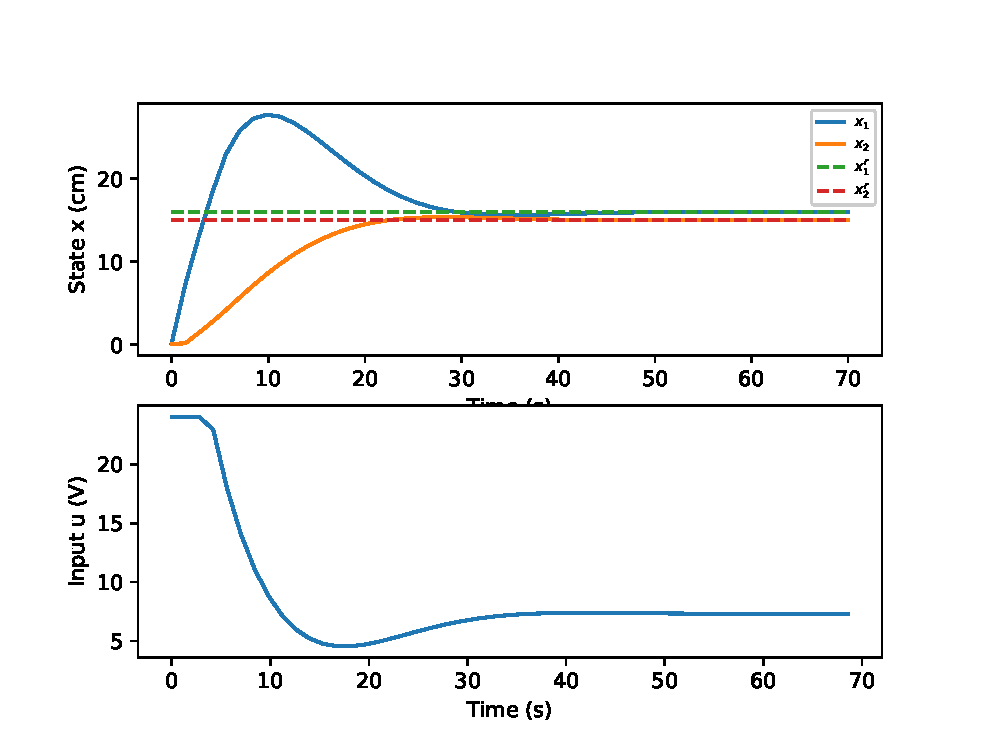
\includegraphics[width=0.45\textwidth]{img/tmpc1.eps} %{<left> <lower> <right> <upper>}
    \caption{State and input trajectories.}
    \label{fig:tmpc1}
\end{figure}

\begin{figure}[h]
    \centering
    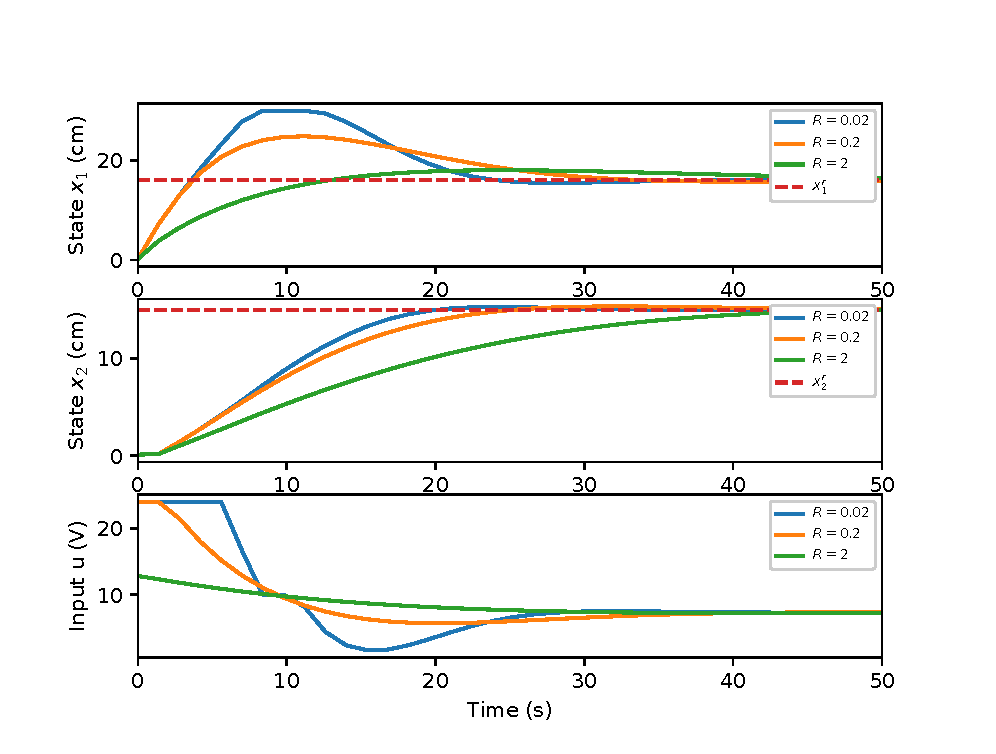
\includegraphics[width=0.45\textwidth]{img/tmpc2.eps} %{<left> <lower> <right> <upper>}
    \caption{Influence of input penalty on the closed-loop response.}
    \label{fig:tmpc2}
\end{figure}

\begin{figure}[h]
    \centering
    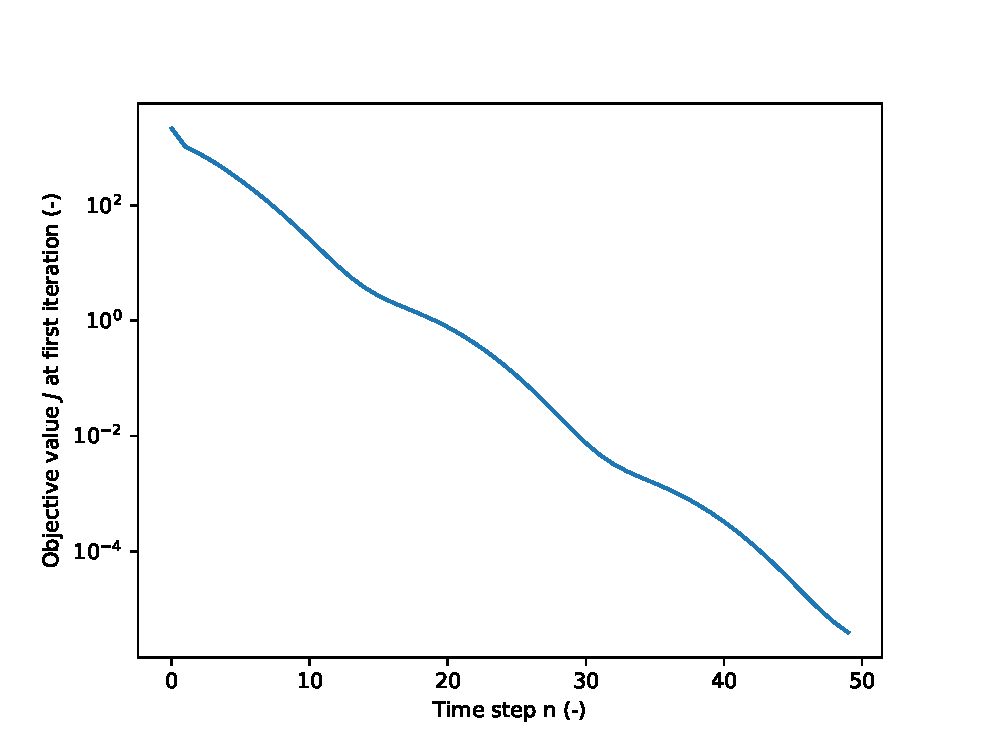
\includegraphics[width=0.45\textwidth]{img/tmpc3.eps} %{<left> <lower> <right> <upper>}
    \caption{Evolution of the objective value at first iteration.}
    \label{fig:tmpc3}
\end{figure}

\begin{figure}[h]
    \centering
    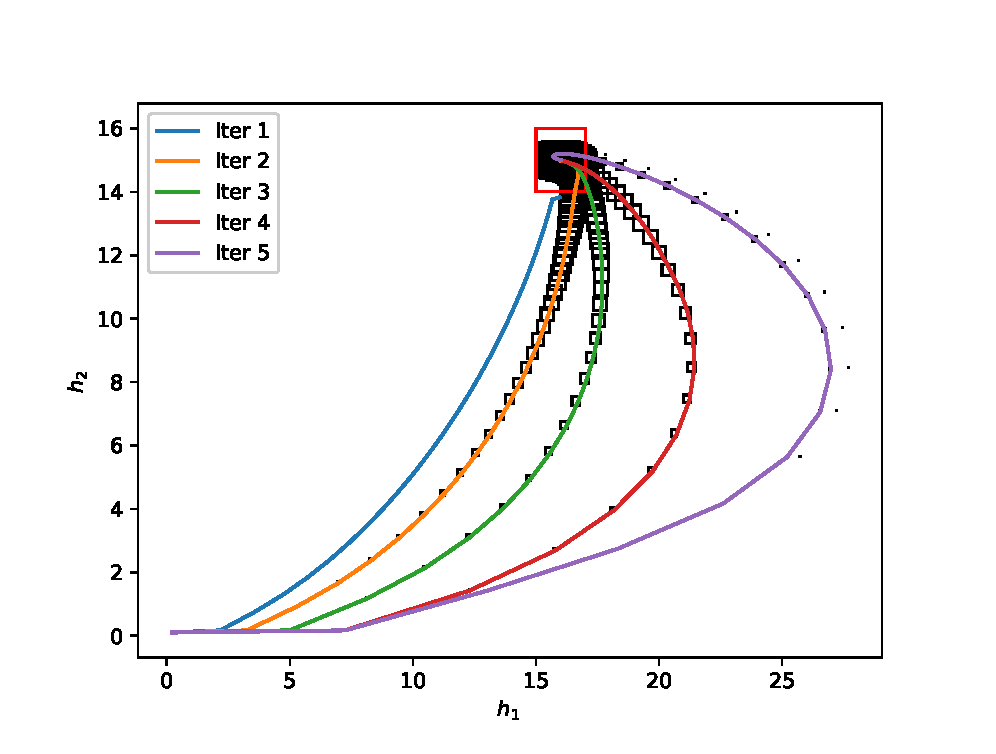
\includegraphics[width=0.45\textwidth]{img/tmpc4.eps} %{<left> <lower> <right> <upper>}
    \caption{Phase portrait at time step $n=0$ with successive predicted state trajectories, associated bounds (black boxes) and terminal set (red box).}
    \label{fig:tmpc4}
\end{figure}


We now compare the convergence properties of DC-TMPC with the successive linearisations tube-based MPC algorithm in \cite{mark} (MPC-2011). As for the present approach, linearisation errors around the successive predicted trajectories are treated as disturbances in MPC-2011. However, bounds on the errors are chosen a priori and do not have the level of flexibility offered by DC-TMPC, which exploits the convex nature of the linearisation errors to find tighter bounds on the state perturbation. As a result, it is expected that DC-TMPC demonstrates faster convergence and a larger feasibility set than MPC-2011. To show that, we adapted the MPC-2011 algorithm for the present coupled tank model and simulated a case study with the same parameters. 
For a given terminal set, the range of open loop input voltage allowable for initialising the algorithm with a feasible problem was found to be $[6.1, 9.3]$ V for DC-TMPC, while it was limited between $[7.2, 7.8]$ V for MPC-2011, showing a smaller feasibility set. This demonstrates the relative conservativeness of the state perturbation bounds in MPC-2011 over DC-TMPC, as expected. Finally, the faster convergence of DC-TMPC is shown in Figure \ref{fig:tmpc5} comparing the evolution of the objective value for both algorithms at the first time step. This achieves to demonstrate the superiority of DC-TMPC over the state-of-the-art MPC-2011 tube-based MPC algorithm with successive linearisations.  

\begin{figure}[h]
    \centering
    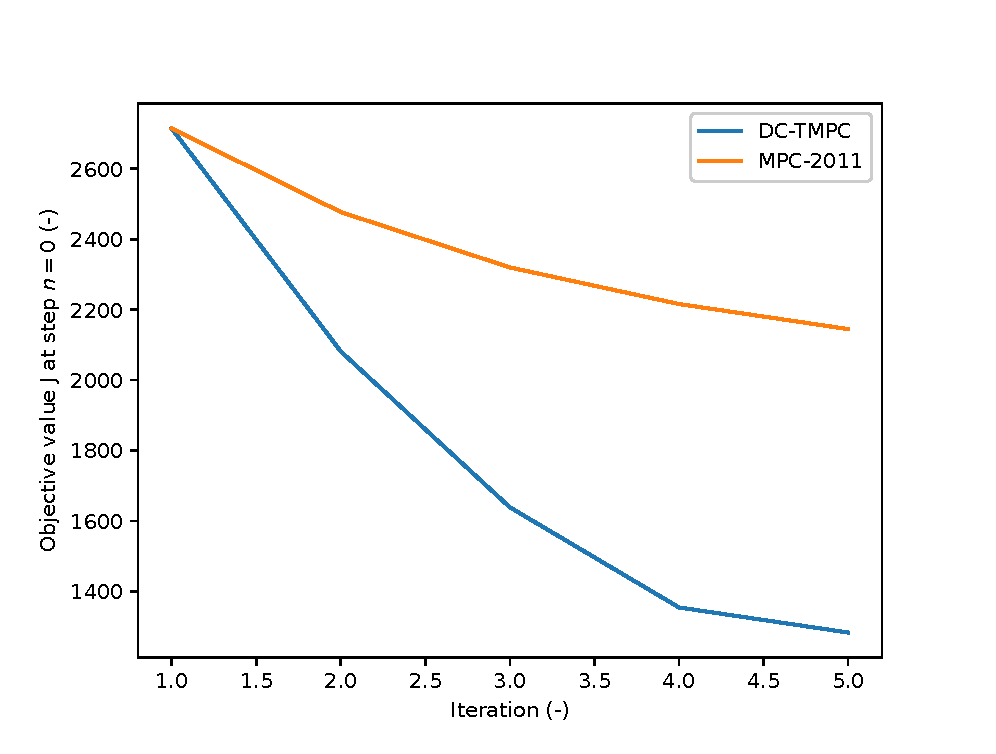
\includegraphics[width=0.45\textwidth]{img/tmpc5.eps} %{<left> <lower> <right> <upper>}
    \caption{Comparison of the objective value for both algorithms.}
    \label{fig:tmpc5}
\end{figure}

\section{Conclusion}
\label{sec:conclusion}

This paper introduces DC-TMPC, a new paradigm for robust nonlinear MPC applied to systems representable as a difference of convex functions. The method relies on successive linearisations of the dynamics around predicted trajectories and exploits convexity in the linearisation errors to construct robust and non-conservative tubes in which the perturbed trajectories lie. Convergence, recursive feasibility and asymptotic stability of the proposed algorithm were demonstrated. The algorithm was then applied to regulation of fluid levels in a coupled tank system. 

Extensions include generalisation of the method to robustly stabilise the system in the presence of (additive) external disturbances, use of other parameterisations of the tube (e.g. ellipsoids or polytopes), application to other systems representable as a difference of convex functions (e.g. the Fermi-Pasta-Ulam oscillator) and inclusion of the state feedback matrix $K_k$  in the optimisation to control the size of the tube online.  

%Another extension would be to investigate the application of DC-TMPC to a broader class of systems whose dynamics are two-times continuously differentiable. Indeed, $C^2$ functions can be decomposed as a difference of convex functions and the DC-TMPC paradigm could be applied. This requires to find a DC decomposition that  minimises conservativeness of the generated tube, which might prove challenging. In particular, functions that admit a piecewise definition in terms of convex and concave functions (e.g. $f(x) = x^3$ or the restriction of $f(x) = \sin(x)$ to the interval $x \in [-\pi/2, \pi/2]$) can be naturally decomposed as a difference of convex functions for which the DC-TMPC algorithm could be applied. 

\bibliography{biblio} 
\bibliographystyle{ieeetr}

\appendix
We present here a SDP optimisation problem to compute the terminal gain $\hat{K}$, cost $Q_N$ and bound $\hat{\gamma}$ associated to state and input square terminal sets of respective side length $2\delta^x$ and  $2\delta^u$. 

@ Mark 
\end{document}
